\section{Segunda Iteración y Resultado Final}
%
En la segunda iteración se utilizó el mapa de $C_D$ para la admisión y escape
como dato de entrada de ICESym.
%
Con esto se realizó una serie de corridas de
optimización con el algoritmo genético, de las cuales se seleccionaron los
mejores candidatos.
%
Se obtuvieron 3 candidatos principales, indicados como \emph{$run_{34}$},
\emph{$run_{38}$}, \emph{$run_{51}$} cuyas geometrías se indican en la
tabla~\ref{tab:2iter_geom}.
%
Se ve que los diámetros son similares y que la mayor variación se da en los
largos de los conductos de admisión y escape.
%
% Exceptuando la corrida $run_{51}$ los ángulos de apertura de los puertos de
% admisión se mantienen cercanos Figura \ref{fig:2iter_general}.
%
Para determinar cuál de todos es el más prometedor, se compararon las curvas de
presión, torque y potencia, las cuales se muestran en la
Figura~\ref{fig:PoTi_segunda_op}.

\begin{table}
\centering
\begin{tabular}{ccccccccc} \toprule
  Corrida & DTA  & DTE  & LIT    & LET    & IIA   & IFA   & EIA   & EFA \\
  -       & mm   & mm   & m      & m      & gra   & gra   & gra   & gra \\ \midrule
  run 34  & 83,2 & 100  & 0,6839 & 1,2323 & 5,81  & 52,26 & 81,29 & 8,71 \\
  run 38  & 83,2 & 96,1 & 1,1226 & 1,1226 & 0     & 52,26 & 87,1  & 8,71 \\
  run 51  & 84,5 & 81,9 & 0,6839 & 0,3548 & 17,42 & 55,16 & 66,77 & 37,74 \\\bottomrule
\end{tabular}
\caption{Geometrías de segunda iteración}\label{tab:2iter_geom}
\end{table}

\begin{figure}[ht]
  \centering
  \begin{subfigure}[b]{.5\textwidth}
    \centering
    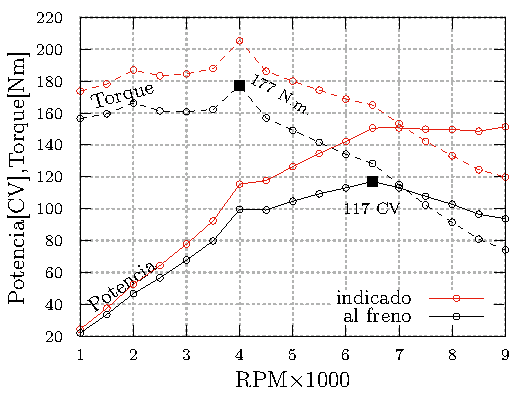
\includegraphics{gnuplot/segunda_iter_pot.pdf}
    \caption{Potencia indicada y al freno} \label{fig:primer_op}
  \end{subfigure}%
  \begin{subfigure}[b]{.5\textwidth}
    \centering
    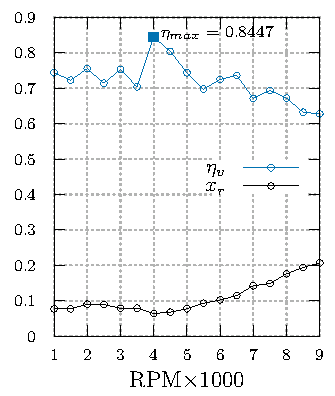
\includegraphics{gnuplot/segundo_rend_vol.pdf}
    \caption{Rendimiento Volumétrico}
  \end{subfigure}
    \caption{Segunda Iteración} \label{fig:primer_op}
\end{figure}


El motor tiene una potencia máxima de 117 CV a las 6500 RPM y un par máximo de
177Nm a 4000 RPM.
%
Este coincide con el máximo de rendimiento volumétrico de $\sim 0,845$.
%
En la Figura~\ref{fig:PoTi_segunda_op} se notan los efectos del coeficiente de
descarga en la simulación del motor, comparando los resultados de la primera
iteración con coeficientes de descarga constantes a la segunda con el mapa de
$C_{D}$ en función de la presión y grado de apertura del puerto.

\begin{figure}[ht]
  \centering
  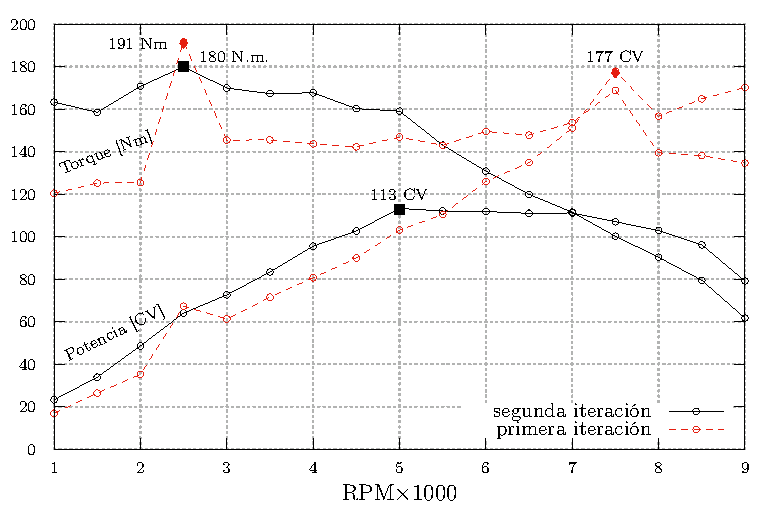
\includegraphics{gnuplot/comparativa.pdf}
  \caption{Comparativa de Torque y potencia al freno} \label{fig:PoTi_segunda_op}
\end{figure}
